%\chapter{Enhancement to Robustness and Generalization}\label{chap:advtraining}

\chapter{Enhancement to Safety and Security of Deep Learning}\label{chap:advtraining}

Significant efforts from the research community have been spent on studying various methods to enhance either the training process or a trained model to mitigate the identified safety risks. In this chapter, we present three representative examples from three categories of techniques. They are designed to deal with different safety risks: robustness, generalisation, and privacy, respectively.  
%
The first category of techniques (Section~\ref{sec:advtrainingsection}), called adversarial training, is to improve the robustness. While there are many different approaches for the improvement of robustness, adversarial training is shown to be the most successful one. We will re-cap the typical min-max formalism of adversarial training, and then discuss some state-of-the-art training techniques. 
%
The second category of techniques (Section~\ref{chap:generalisationPAC}) is to improve the generalisation ability of a trained neural network. The technique presented, based on PAC Bayesian theory, utilises the weight correlation -- a novel concept that measures the correlation between weights of the same layer -- for training. 
%
The third category of techniques (Section~\ref{sec:privacyenhancementsec}) is to improve the privacy-related properties, such as membership inference, model stealing, and model inversion. They are based on differential privacy, and add random noise into either the training process or the inference stage. 

\section{Robustness Enhancement through Min-Max Optimisation}\label{sec:advtrainingsection}



Deep neural networks (DNNs) can be easily fooled to confidently make incorrect predictions by adding small and human-imperceptible perturbations to their input~\cite{DBLP:journals/corr/GoodfellowSS14,szegedy2013intriguing,wu2020skip}. The study of adversarial defences, aiming to ultimately eliminate adversarial threat~\cite{kurakin2016adversarial}, has brought about significant advances in the past few years, with various techniques developed, including input denoising~\cite{bai2019hilbert}, adversarial detection~\cite{ma2018characterizing}, gradient regularisation~\cite{tramer2017ensemble}, feature squeezing~\cite{xu2017feature}, defensive distillation~\cite{papernot2016distillation} and adversarial training~\cite{madry2017towards,papernot2016distillation}. Among various techniques, adversarial training is known to be the most effective one~\cite{athalye2018obfuscated}.

Adversarial training
considers adversarial examples during the training. Consider a training dataset $D_{train}=\{(\mathbf{x}_i,y_i)\}_{i=1}^m$ with $m \in \mathbb{N}$ samples drawn from a distribution $\mathcal{D}$, where $\mathbf{x}_i \in \mathbb{R}^d$ is an example in the $d$-dimensional input space and $y_i$ is its ground-truth label, adversarial training~\cite{madry2017towards} updates the minimisation objective of the  training scheme from the usual one as follows 
\begin{equation}
J=\mathop{\mathbb{E}}\limits_{(\mathbf{x},y)\sim \mathcal{D}}  \mathcal{L}(\mathbf{x};y;f_\theta)
\label{eq0}
\end{equation}
to 
\begin{equation}
     J_{\mathrm{adv}}=\mathop{\mathbb{E}}\limits_{(\mathbf{x},y)\sim \mathcal{D}} \bigg[\max_{||\mathbf{x}'-\mathbf{x}||_p\le \epsilon} \mathcal{L}(\mathbf{x}';y;f_\theta)\bigg],
\label{eq1}
\end{equation}
where $\mathbf{x}'$ is the adversarial example within the $\epsilon$-ball (bounded by an $\ell_p$-norm) centred at clean example $\mathbf{x}$, $f_\theta(\cdot)$ is the DNN with parameter $\theta$, and $\mathcal{L}(\cdot)$ is the standard classification loss (e.g., the cross-entropy loss). 
Therefore, adversarial training is formulated as a min-max optimisation problem.



%[Below are old Contents in the deep learning chapter, check to see if they are needed, or integrate with the above]

On the opposite side of adversarial attacks~\cite{biggio2013evasion, szegedy2014intriguing}, researchers also show huge interest in designing various defence techniques, which are to either identify or reduce adversarial examples so that the decision of the DNN can be more robust. Until now, the developments of attack and defence techniques have been seen as an ``arm-race''. For example, most defences against attacks in the white-box setting, including~\cite{hendrycks2016early,meng2017magnet,metzen2017detecting,papernot2016distillation}, have been demonstrated to be vulnerable to e.g., iterative optimisation-based attacks~\cite{carlini2017adversarial,carlini2017magnet}.
%Here we only cover a few works that are relevant to . 
%review some notable works that are recently emerged.



%\subsection{Training with Adversarial Examples}

%\subsection{Label Smoothing}

\subsection{Normal Adversarial Training}

% Adversarial training proposed in \cite{FGSM} proceeds by training on adversarial examples until the model learns to classify them correctly.
% %
% Given a training dataset $D$ and a loss function $\mathcal{L}(\cdot)$, standard training chooses network weights $\theta$ as 

Adversarial training is one of the most notable defence methods, which was first proposed by~\cite{DBLP:journals/corr/GoodfellowSS14}. It can improve the robustness of DNNs against adversarial attacks by retraining the model on adversarial examples. Its basic idea can be expressed as below:
\begin{equation}
\theta^* = \arg \min_\theta\; \mathop{\mathbb{E}}\limits_{(\mathbf{x},y)\sim \mathcal{D}} \; \mathcal{L}(\mathbf{x}; y; f_\theta).
\end{equation}
%where $f_\theta$ is a DNN parameterized by $\theta$, $\mathcal{L}(\cdot)$ is the loss function, $D$ is the training dataset.
This is improved in \cite{madry2017towards} by assuming that all neighbours within the $\epsilon$-ball should have the same class label, i.e., local robustness. Technically, this is done by changing the optimisation problem by requiring that   
%
%adversarial training approach of \cite{madry2017towards} is, 
for a given $\epsilon$-ball (represented as a $d$-Neighbourhood), to solve \begin{equation}
\label{eq_advtrn}
\theta^* = \arg \min_\theta\; \mathop{\mathbb{E}}\limits_{(\mathbf{x},y)\sim \mathcal{D}} \left[ \max_{||\mathbf{x}'-\mathbf{x}||_p\le \epsilon} \mathcal{L}(\mathbf{x}'; y; f_\theta) \right].
\end{equation} 
%Intuitively, it is to assume that all neighbours within the $\epsilon$-ball should have the same class label and should be considered during the training. 
% An approximate algorithm is suggested to 
% %approximately solve this formulation, the authors 
% solve the inner maximization problem by generating adversarial examples using projected gradient descent (PGD).
\iffalse
%Adversarial training is an effective approach to improve the robustness of a deep learning model. 
The general idea is to create and incorporate adversarial examples into the training process. Surely, given there are many different ways of generating adversarial examples and various ways of incorporating them into training, this general idea thus can be implemented in a variety of approaches. 
%
The following is a typical format on how to conduct adversarial training.  
%
\begin{equation}
    \min_{\textbf{W}} \sum_{(\textbf{x},y)\in D} \max_{\textbf{\textdelta} \in \Delta(\textbf{x})} L(f_{\textbf{W}}(\textbf{x}+\textbf{\textdelta}),y)
\end{equation}
\fi
%
Intuitively, it is a min-max process, where each learning batch is conducted by first selecting the worst-case adversarial perturbation during the \emph{inner maximisation}, and then adapting weights to reduce the loss by the adversarial perturbation in \emph{outer minimisation}. \cite{madry2017towards} adopted Projected Gradient Descent (PGD) to approximately solve the inner maximisation problem.
Please see the template code in Section~\ref{sec:competitionresilience} for the adversarial training. 

% Aiming at defending iterative attacks, 
% cascade adversarial machine learning \cite{na2017cascade} is proposed to generate adversarial examples at each mini-batch. Technically, it trains a first model, generates adversarial examples (with iterative attack methods) on that model, adds these to the training set, then trains a second model on the augmented dataset, and so on.
Later on, to defeat the iterative attacks, \cite{na2017cascade} proposed to use a cascade adversarial method which can produce adversarial images in every mini-batch. Namely, at each batch, it performs a separate adversarial training by putting the adversarial images (produced in that batch) into the training dataset.
%Additionally, the authors construct a ``unified embedding'' and enforce
%that the clean and adversarial logits are close under some metric.
Moreover,~\cite{tramer2017ensemble} introduces ensemble adversarial training, which augments training data with perturbations transferred from other models. 


\subsection{State-of-the-art Adversarial Training Technology}
The first category is to reduce Equation~\ref{eq_advtrn} to an equivalent, or approximate, expression, which includes measuring the distance between $\mathbf{x}$ and $\mathbf{x}'$.
For example, ALP~\cite{engstrom2018evaluating,kannan2018adversarial} enforces the similarity between $f_\theta(\mathbf{x})$ and $f_\theta(\mathbf{x'})$, the logits activations on unperturbed and adversarial versions of the same input $\mathbf{x}$.
MMA~\cite{ding2018mma} encourages every correctly classified instance $\mathbf{x}$ to leave a sufficiently large margin, i.e., the distance to the boundary, by maximising the size of the shortest successful perturbation. 
MART~\cite{wang2019improving} observes the difference between misclassified and correctly classified examples in adversarial training, and suggests different loss functions for them. 
TRADES~\cite{zhang2019theoretically} analyses the robustness error and the clean error, and shows an upper bound and lower bound on the gap between robust error and clean error, which motivates adversarial training networks to optimise with
\begin{equation}
\mathcal{L}(\mathbf{x}; y; f_\theta)+\mathrm{KL}\big(f_\theta (\mathbf{x})||f_\theta (\mathbf{x}')\big)/\lambda,
\end{equation}
where $\lambda$ is the hyper-parameter to control the trade-off between clean accuracy and robust accuracy. 
It considers the $\mathrm{KL}$-divergence of the activations of the output layer, i.e., $\mathrm{KL}(f_\theta(\mathbf{x})||f_\theta(\mathbf{x}'))$, for every instance $\mathbf{x}$.
The measurement over $\mathbf{x}$ and $\mathbf{x}'$ can be extended to consider a local distributional distance, i.e., the distance between the distributions within a norm ball of $\mathbf{x}$ and within a norm ball of $\mathbf{x}'$. 
For example, \cite{Zheng_Chen_Ren_2019} forces the similarity between local distributions of an image and its adversarial example, \cite{SJ2017} uses Wasserstein distance to measure the similarity of local distributions, and  \cite{dong2020adversarial,NEURIPS2020_5de8a360,dong2020benchmarking,mao2019metric,pang2020bag} optimise over distributions over a set of adversarial perturbations for a single image.





The second category is to pre-process the generated adversarial examples before training instead of directly using the adversarial examples generated by attack algorithms.
Notable examples include label smoothing~\cite{chen2020robust,szegedy2016rethinking}, which, instead of considering the adversarial instances $(\mathbf{x}',y)$ for the ``hard'' label $y$, it consider $(\mathbf{x}',\mathbf{\tilde{y}})$, where $\mathbf{\tilde{y}}$ is a ``soft'' label represented as a weighted sum of the hard label and the uniform distribution. 
This idea is further exploited in ~\cite{muller2019does}, which empirically studies how label smoothing works.
Based on these, AVMixup~\cite{lee2020adversarial,zhang2020does} defines a  virtual sample in the adversarial direction and extends the training distribution with soft labels via linear interpolation of the virtual sample and the clean sample.
Specifically, it optimises 
\begin{equation}
\mathcal{L}(\mathbf{\check x},\mathbf{\check y}, f_\theta),
\end{equation}
where $\mathbf{\check x}=\beta\mathbf{x}+(1-\beta)\gamma(\mathbf{x}'-\mathbf{x})$, $\mathbf{\check y}=\beta\phi(\mathbf{y},\lambda_1)+(1-\beta)\phi(\mathbf{y},\lambda_2)$, 
$\beta$ is drawn from the Beta distribution for each single $\mathbf{x}_i$, $\gamma$ is the hyper-parameter to control the scale of adversarial virtual vector, $\textbf{y}$ is the one-hot vector of $y$,  $\phi(\cdot)$ is the label smoothing function~\cite{szegedy2016rethinking}, and $\lambda_1$ and $\lambda_2$ are hyper-parameters to control the smoothing degree. 
Other than label smoothing, \cite{NEURIPS2019_d8700cbd} generates adversarial examples by perturbing the local neighbourhood structure in an unsupervised fashion.


These two categories follow the min-max formalism and only adapt its components. AWP~\cite{wu2020adversarial} adapts the inner maximisation to take one additional maximisation to find a weight perturbation based on the generated adversarial examples. The outer minimisation is then based on the perturbed weights~\cite{devries2017improved} to minimise the loss induced by the adversarial examples.
Specifically, it is to optimise the double-perturbation adversarial training problem
\begin{equation}
\label{eq_awp}
    \max_{\vec{V}\in\mathcal{V}}\mathcal{L}( f_{\theta+\vec{V}}(\mathbf{x}') ),
\end{equation}
where $\mathcal{V}$ is a feasible region for the parameter perturbation~$\vec{V}$. 


In addition, \cite{zhang2019theoretically} regularises the output of natural inputs and corresponding adversarial examples (generated by PGD attack) with the KL divergence. \cite{xie2019intriguing} explores the normalisation in adversarial training and studies the Mixture batch normalisation mechanism by using respective batch normalisation layers for natural data and adversarial examples. \cite{cui2021learnable} proposes the Learnable Boundary Guided Adversarial Training (LBGAT) method, to improve robustness without losing much natural accuracy. \cite{jin2022enhancing} regularises second-order statistics of weights to improve robustness with the theoretical support from PAC-Bayesian adversarial bound.  
























\section{Generalisation Enhancement through PAC Bayesian Theory}\label{chap:generalisationPAC}


Since the invention of the PAC-Bayesian framework~\cite{mcallester1999pac}, there have been a number of canonical works developed in the past decades, including the parametrisation of the PAC-Bayesian bound with Gaussian distribution~\cite{langford2002not,langford2003pac}, the early works about generalisation error bounds for learning problems~\cite{germain2009pac,maurer2004note,parrado2012pac,welling2011bayesian} and the recent works about PAC-Bayes for machine learning models~\cite{alquier2016properties,blundell2015weight,dwork2015generalization,dwork2015preserving,dziugaite2018data,letarte2019dichotomize,perez2021tighter,rivasplata2019pac,thiemann2017strongly}. In the following, we will present a novelty method to improve DNN's generalisation performance through PAC-Bayesian theory.   


Given a prior distribution over the parameter $\theta$, which is selected before seeing a training dataset, a posterior distribution on $\theta$ will depend on both, the training dataset and a specific learning algorithm. The PAC-Bayesian framework~\cite{mcallester1999pac} bounds the generalisation error with respect to the KL divergence~\cite{KL1951} between the posterior and the prior distributions.


Consider a training dataset $D_{train}$ with $m \in \mathbb{N}$ samples drawn from a distribution $\mathcal{D}$. Given a learning algorithm (e.g., a classifier) $f_\theta$ with prior and posterior distributions $P$ and $Q$ on the parameter $\theta$ respectively, 
for any $\delta > 0$,
with probability $1-\delta$ over the draw of training data, we have that~\cite{dziugaite2017computing,mcallester1999pac} 
\begin{equation}
\label{eq:pac}
\mathbb{E}_{\theta \sim Q}[\mathcal{L}_\mathcal{D}(f_\theta)]\le \mathbb{E}_{\theta \sim Q}[\mathcal{L}_{D_{train}}(f_\theta)] + \sqrt{\frac{\mathrm{KL}(Q || P)+\log \frac{m}{\delta}}{2(m-1)}},
\end{equation}
where $\mathbb{E}_{\theta \sim Q}[\mathcal{L}_\mathcal{D}(f_\theta)]$ is the expected loss on $\mathcal{D}$, $\mathbb{E}_{\theta \sim Q}[\mathcal{L}_{D_{train}}(f_\theta)]$ is the empirical loss on $D_{train}$, and their difference yields the generalisation error. Equation~\ref{eq:pac} outlines the role KL divergence plays in the upper bound of the generalisation error. In particular, a smaller KL term will help tighten the generalisation error bound.  
Assume that $P$ and $Q$ are Gaussian distributions with $P=\mathcal{N}(\mu_P,\Sigma_P)$ and $Q=\mathcal{N}(\mu_Q,\Sigma_Q)$, then the
$\mathrm{KL}$-term can be written as follows:
\begin{equation}
\label{formula4}
\begin{aligned}
    &\mathrm{KL}(\mathcal{N}(\mu_Q,\Sigma_Q)||\mathcal{N}(\mu_P,\Sigma_P))\\
    &=\frac{1}{2}\Big[ \mathrm{tr}(\Sigma_P^{-1} \Sigma_Q)+(\mu_Q-\mu_P)^\top \Sigma_P^{-1}(\mu_Q-\mu_P)-k+\ln{\frac{\mathrm{det}\Sigma_P}{\mathrm{det}\Sigma_Q}} \Big],
\end{aligned}
\end{equation}
where $k$ is the number of parameters in $\theta$. Below, \cite{jin2020does}  incorporates weight correlation into this framework to tighten the bound. 


\subsection*{Weight Correlation in Fully Connected Neural Network (FCN).} Given weight matrix $w_l \in \mathbb{R}^{N_{l-1} \times N_l}$ of the $l$-th layer ($N_l$ is the number of neurons of the $l$-th layer), the average weight correlation of FCN is defined as
\begin{equation}
    \rho(N_l) =\frac{1}{N_l(N_l-1)} \sum_{i,j=1 \atop i \ne j}^{N_l} \frac{|w_{l i}^T w_{l j}|}{||w_{l i}||_2 ||w_{l j}||_2},
\end{equation}
where $w_{l i}$ and $w_{l j}$ are $i$-th and $j$-th column of the matrix $w_l$, corresponding to the $i$-th and $j$-th neuron at $l$-th layer, respectively.  Intuitively, $\rho(w_l)$ is the average cosine similarity between weight vectors of any two neurons at $l$-th layer.


\subsection*{Weight Correlation in  Convolutional Neural Network (CNN).} Given the filter tensor $w_l \in \mathbb{R}^{c \times c \times N_{l-1} \times N_l}$ of the $l$-th layer, where $c \times c$ is the size of the convolution kernel, $w_{l i} \in \mathbb{R}^{c \times c \times N_{l-1}}$ and $w_{l j} \in \mathbb{R}^{c \times c \times N_{l-1}}$ are the $i$-th and $j$-th filter, respectively, of the filter tensor $w_l$. By reshaping $w_{l i}$ and $w_{l j}$ into $w'_{l i} \in \mathbb{R}^{c^2 \times N_{l-1}}$ and $w'_{l j} \in \mathbb{R}^{c^2 \times N_{l-1}}$, respectively, the weight correlation of CNN is defined as
\begin{equation}
    \rho(w_l)=\frac{1}{N_l(N_l-1)N_{l-1}} \sum_{i,j=1 \atop i \ne j}^{N_l}  \sum_{z=1}^{N_{l-1}}\frac{|{w'}_{l i,z}^T{w'}_{l j,z}|}{||w'_{l i,z}||_2 ||w'_{l j,z}||_2},
\end{equation}
where $w'_{l i,z}$ and $w'_{l j,z}$ are the $z$-th column   of $w'_{l i}$ and $w'_{l j}$ respectively. Intuitively, $\rho(w_l)$ is defined as the cosine similarity between filter matrices.

\begin{figure}[t!]
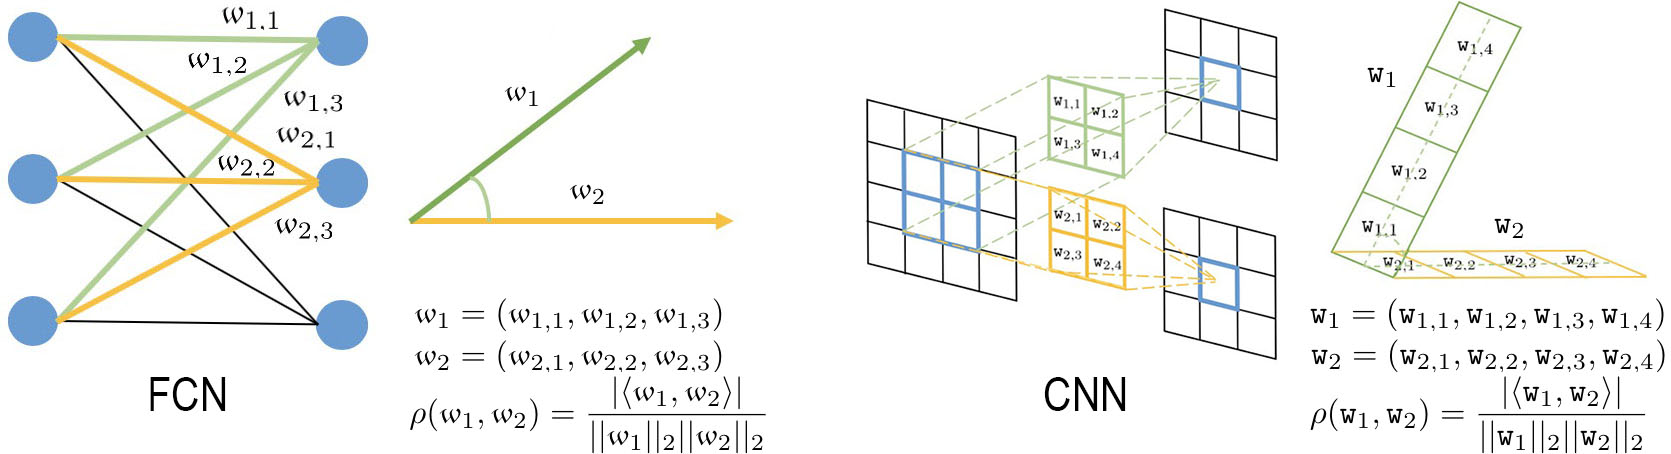
\includegraphics[width=1
\textwidth]{images/PAC-Bayes/figure3.jpg}
\centering
%\vspace{-2mm}
\caption{\textbf{(FCN)} The weight correlation of any two neurons is the cosine similarity of the associated weight vectors. \textbf{(CNN)} The weight correlation of any two filters is the cosine similarity of the reshaped filter matrices.}    
\vspace{-4mm}
\label{fig:definitions}
\end{figure}

Considering the above $\rho(w_l)$, \cite{jin2020does} introduces a correlation matrix $\Sigma_{\rho(w_l)} \in \mathbb{R}^{N_l \times N_l}$, with diagonal elements being $1$, and off-diagonal ones all $\rho(w_l)$. Then, the posterior corvariance matrix can be represented as $\Sigma_{Q_{w_l}}=\Sigma_{\rho(w_l)} \otimes \sigma_l^2I_{N_{l-1}}$, where $\otimes$ is Kronecker product. Let $g(w)=\sum g(w_l)$ where $g(w_l)$ defined by:
\begin{align}
     g(w_l)
     &= - (N_l-1)N_{l-1} \ln (1-\rho(w_l)) - N_{l-1} \ln(1+(N_l-1)\rho(w_l)).
\end{align}
Then the KL term w.r.t. the $l$-th layer can be given by
\begin{equation}
\label{eq:packl}
\begin{aligned}
\mathrm{KL}(Q || P)_l=\frac{||\theta_l^F-\theta_l^0||_{\mathrm{Fr}}^2}{2\sigma_l^2} + g(w_l),
\end{aligned}
\end{equation}
where $\theta^0$ and $\theta^F$ refer to the value of parameters at initialisation and at the end of training, respectively. Further, when $\sigma_l^2=\sigma^2$ for all $l$, we have $\mathrm{KL}(Q || P) = \sum_{l=1}^L \mathrm{KL}(Q || P)_l$. Given the above derivation, \cite{jin2020does} concludes that the KL term in Equation~\ref{eq:packl} is positively correlated to $g(w_l)$. Naturally, $g(w_l)$ can be considered as a regulariser term in the training function.

The training of a neural network is seen as a process of optimising over an objective function $J(\theta;\textbf{x},y)$. \cite{jin2020does} adds a penalty term $g(w)=\sum_{l} g(w_{l})$, which is a function of $\rho(w)$, to the objective function $J$, and denote the regularised objective function by $\tilde{J}$:
\begin{equation}
    \tilde{J}(\theta;\textbf{x},y) = J(\theta;\textbf{x},y) + \alpha g(w),
\end{equation}
where $\alpha \in [0,\infty)$ is a hyper-parameter that balances the relative contribution of the $g(w_l)$ penalty term. Figure~\ref{fig2} provides an illustrative diagram to show the utility of the regularisation. This regularisation is an effective and computationally efficient tool to enhance generalisation performance in practice~\cite{jin2020does}, which could complement other commonly used regularisers such as weight decay and dropout.  

\begin{figure}[t!]
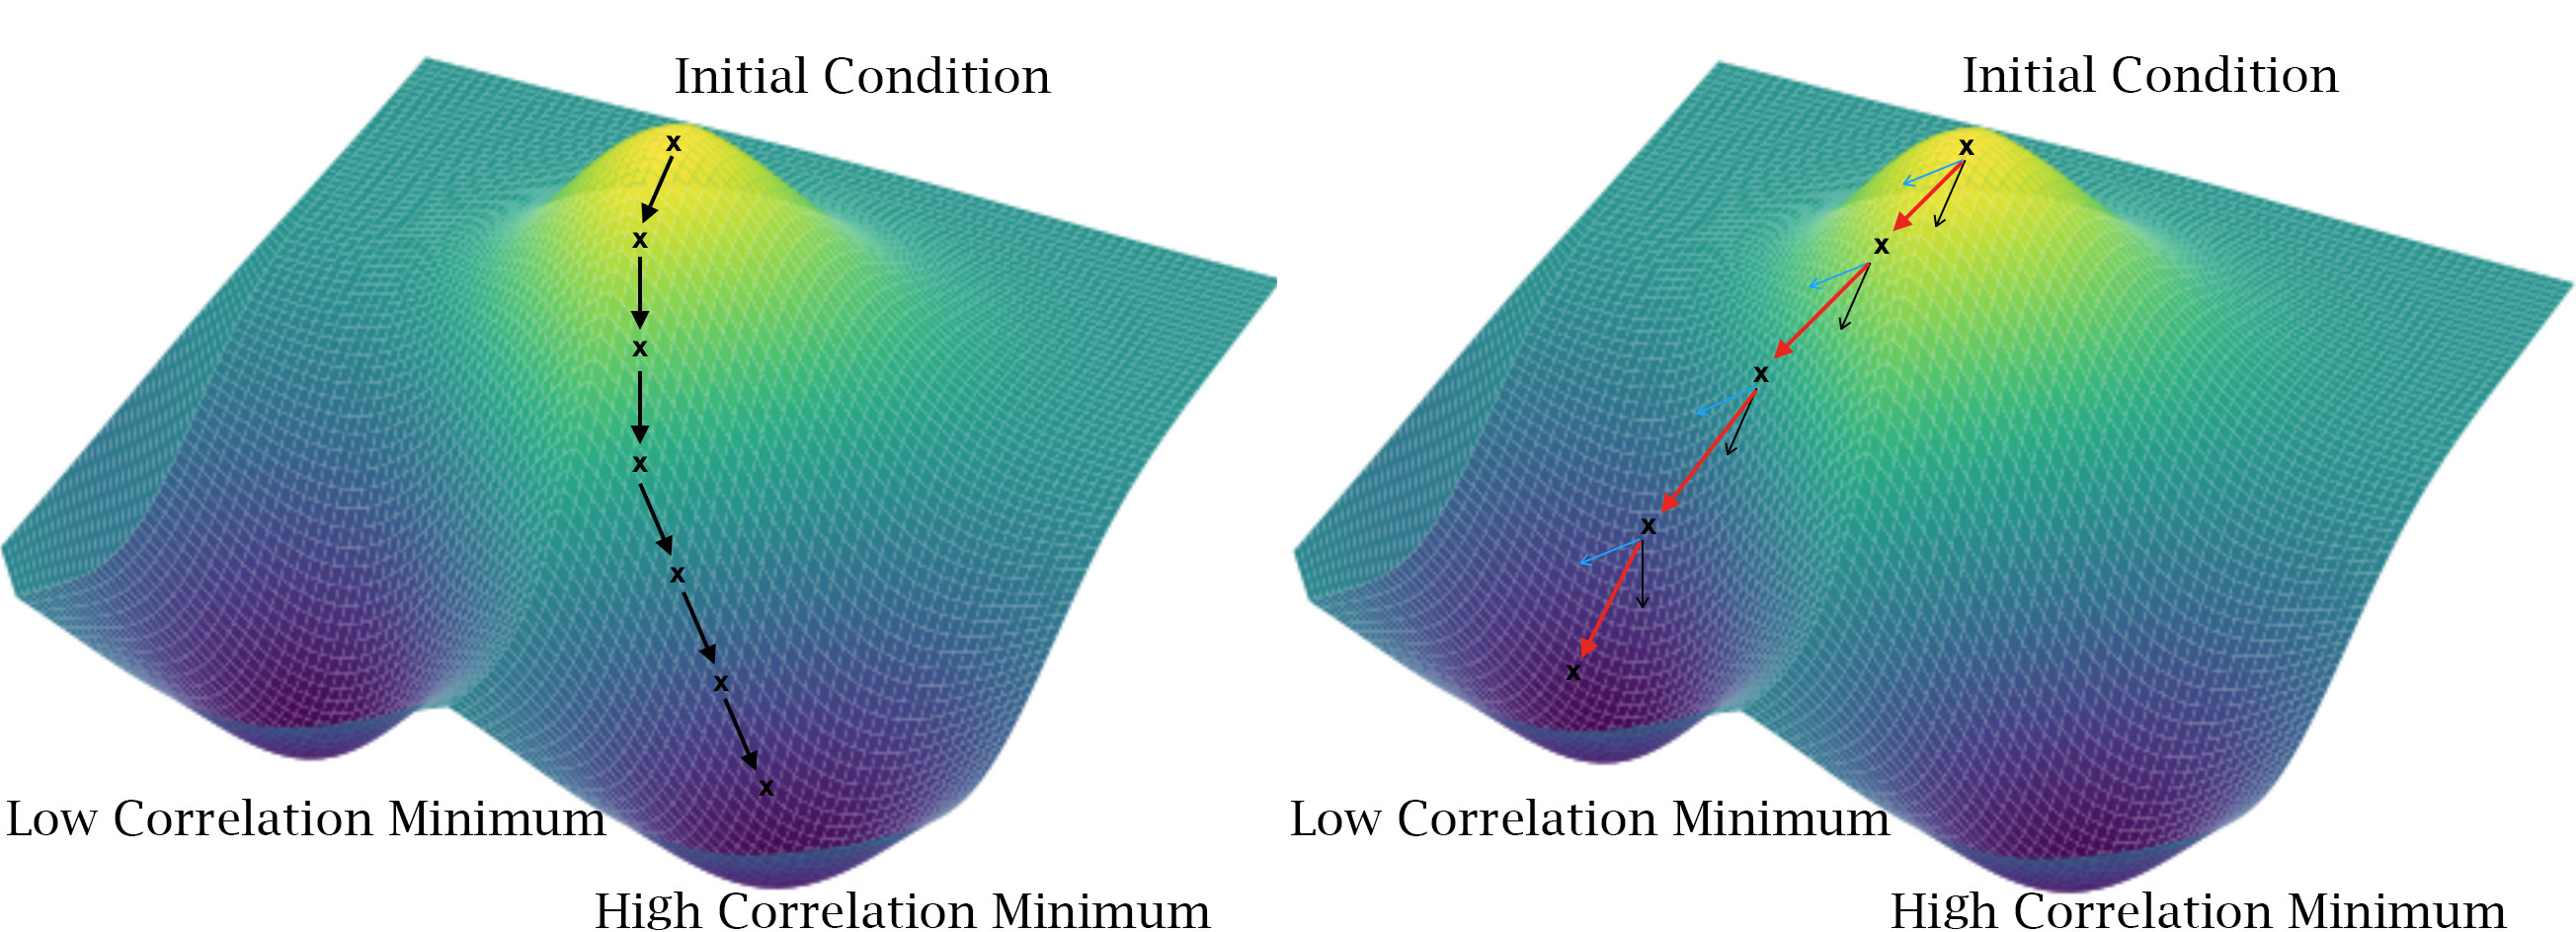
\includegraphics[width=1
\textwidth]{images/PAC-Bayes/figure2_2.jpg}
\centering
%\vspace{-4mm}
\caption{\textbf{Left}: Normal gradient-based optimisers may find a local minimum with high correlation.  \textbf{Right}: Weight correlation regularisation helps the optimiser to find a low correlation minimum, which is more likely to be a global minimum.}    
\vspace{-4mm}
\label{fig2}
\end{figure}


\section{Privacy Enhancement through Differential Privacy}\label{sec:privacyenhancementsec}

We have presented in Chapter~\ref{sec:defsafetyissues} several security properties related to the leakage of privacy information, including membership inference and model inversion, and then discussed some algorithms that exploit different machine learning algorithms for privacy leakages, for example Chapters \ref{sec:membershipInferenceDL} and \ref{sec:modelInversionDL} for deep learning algorithms. In this section, we consider how to enhance machine learning algorithms so that they may perform better in protecting the privacy information.

A straightforward idea for privacy protection is the naive anonymisation, by removing sensitive features such as names, addresses, and postcodes from the data. Unfortunately, an adversary can identify the user and uncover potentially sensitive information through  auxiliary knowledge. For example, \cite{4531148} shows that for machine learning model trained on Netflix Prize dataset, the attack can utilise auxiliary knowledge from the publicly available Internet Movie Database records.  

While there are many different methods that have been proposed in the literature, we mainly focus on methods based on differential privacy (DP), because DP provides strong theoretical guarantees. 

\subsection{Differential Privacy}

DP was originally developed when needing to publish aggregate information about a statistical database. It is required that the disclosure of private information of the records in the database is limited. 

Let $\mathcal{A}$ be a randomised algorithm that generates an output according to a database. Let $\mathcal{O}_{\mathcal{A}}$ be the set of possible outputs of  $\mathcal{A}$, and we use $\mathcal{S}$ to range over $\mathcal{P}(\mathcal{O})$, i.e.,  the set of subsets of $\mathcal{O}$. 

\begin{definition}
The algorithm $\mathcal{A}$ is said to provide 
$\epsilon$-differential privacy for $\epsilon$ a non-negative number, if for all datasets $D_1$ and $D_2$ that differ on a single element, we have 
\begin{equation}
    \forall \mathcal{S}\in \mathcal{P}(\mathcal{O}_{\mathcal{A}}):  P(\mathcal{A}(D_1) \in \mathcal{S}) \leq e^{\varepsilon} \cdot P(\mathcal{A}(D_2) \in \mathcal{S})
\end{equation}
\end{definition}

Besides, we may also have $(\epsilon,\delta)$-differential privacy as follows. 
\begin{definition}
The algorithm $\mathcal{A}$ is said to provide 
$(\epsilon,\delta)$-differential privacy for two non-negative numbers $\epsilon$ and $\delta$,  if for all datasets $D_1$ and $D_2$ that differ on a single element, we have 
\begin{equation}
    \forall \mathcal{S}\in \mathcal{P}(\mathcal{O}_{\mathcal{A}}):  P(\mathcal{A}(D_1) \in \mathcal{S}) \leq \delta + e^{\varepsilon} \cdot P(\mathcal{A}(D_2) \in \mathcal{S})
\end{equation}
\end{definition}

Intuitively, $\delta$ represents the probability that the algorithm's output varies by more than a factor of $e^{\epsilon}$ when applied to a dataset $D_1$ and any one of its neighbours $D_2$. A smaller $\delta$ suggests a greater confidence and a smaller $\epsilon$ suggests a tighter standard of privacy protection. Actually, the smaller $\delta$ and $\epsilon$ are,  the closer $P(\mathcal{A}(D_1)$ and $P(\mathcal{A}(D_2) \in \mathcal{S})$ is, and therefore, the stronger privacy protection. 

\subsection{Private Algorithms for Training}

While there are different proposals on integrating noises into training process to enhance the privacy protection (and implementing DP), we discuss a simple algorithm, DP-SGD \cite{DBLP:conf/focs/BassilyST14}, that lifts the stochastic gradient descent (SGD) -- the training algorithm for deep learning -- with noise. Typically, the SGD algorithm iterates over minibatchs, such that each minibatch is a small set of training examples. For every minibatch $D$, it updates the weight as follows: 
\begin{equation}
    \theta_{t+1} \leftarrow \theta_t + \eta \nabla_t \mathcal{L}(D;\theta_t)
\end{equation}
where $\eta$ is the learning rate, and $\mathcal{L}(D ;\theta_t)$ is a loss function returning the average loss over the training instances in the minibatch $D$ under the current weights $\theta_t$. For DP-SGD, two modifications are made. First of all, the update is done on individual instances, instead of on a minibatch. Second, every gradient is added with a noise, i.e., 
\begin{equation}
    \theta_{t+1} \leftarrow \theta_t + \eta( \nabla_t \mathcal{L}(\textbf{x};\theta_t)+ b_t)
\end{equation}
where $\textbf{x}$ is a training sample randomly selected from $D_{train}$ and $b_t$ is sampled from a Gaussian noise $\mathcal{N}(0,\sigma^2)$ such that 
\begin{equation}
    \sigma = \sqrt{\frac{32 L^2 n^2 \log(n/\delta)\log (1/\delta)}{\epsilon^2}}
\end{equation}
This update is conducted for $|D_{train}|^2$ times. 
It is proved \cite{DBLP:conf/focs/BassilyST14} that this algorithm is $(\epsilon,\delta)$-differential private. 

\subsection{Model Agnostic Private Learning}

The above algorithm adapts the training algorithm for deep learning. In the following, we consider an algorithm, PATE \cite{DBLP:conf/iclr/PapernotAEGT17}, which does not rely on specific machine learning algorithm. Instead, the noise is added when aggregating results from multiple models trained over the partition of the dataset. Actually, the training dataset $D_{train}$ is split into $k$ datasets $D_{train}^1,...,D_{train}^k$, each of which is used to train a model $f^i$ for $i=1..k$. Then, for each class $j\in C$, we let 
\begin{equation}
    n_j (\textbf{x})= |\{ f^i(\textbf{x})=j ~|~ i=1..k\}|
\end{equation}
be the number of models that predict $\textbf{x}$ as the label $j$. The privacy protected output is 
\begin{equation}
    f(\textbf{x}) = \argmax_{j\in C} (n_j(\textbf{x}) + Lap(\frac{1}{\lambda}))
\end{equation}
where $Lap(b)$ is the Laplacian distribution with location $0$ and scale $b$, and $\gamma$ is a hyper-parameter. Intuitively, a large $\gamma$ suggests a strong privacy guarantee, but may degrade the accuracy.



\newpage 
\Extrachap{Exercises}
%\addcontentsline{toc}{chapter}{\protect\numberline{}Exercises}%

%%% about attack and verification%%%%

\begin{newquestion}{\textbf{1}~~}
Please use an example to demonstrate your understanding of the dissimilarities of adversarial attacks and verification.
\end{newquestion}


\begin{newquestion}{\textbf{2}~~}
Please explain why $L_p$-norm distance metrics are important and how they were normally used in adversarial attacks for image classification models? (You can use one of the well-established attack methods as an example to facilitate the explanation)
\end{newquestion}


\begin{newquestion}{\textbf{3}~~}
Please explain why $L_p$-norm distance metrics are important and how they were normally used in adversarial attacks for image classification models? (You can use one of the well-established attack methods as an example to facilitate the explanation)
\end{newquestion}


\begin{newquestion}{\textbf{4}~~}
In robustness verification, some verification methods are sound, some are both sound and complete, please explain the soundness and completeness in verification. Could you please also name a few verification techniques/tools that are both sound and complete?
\end{newquestion}


\begin{figure}[h]
	\centering
	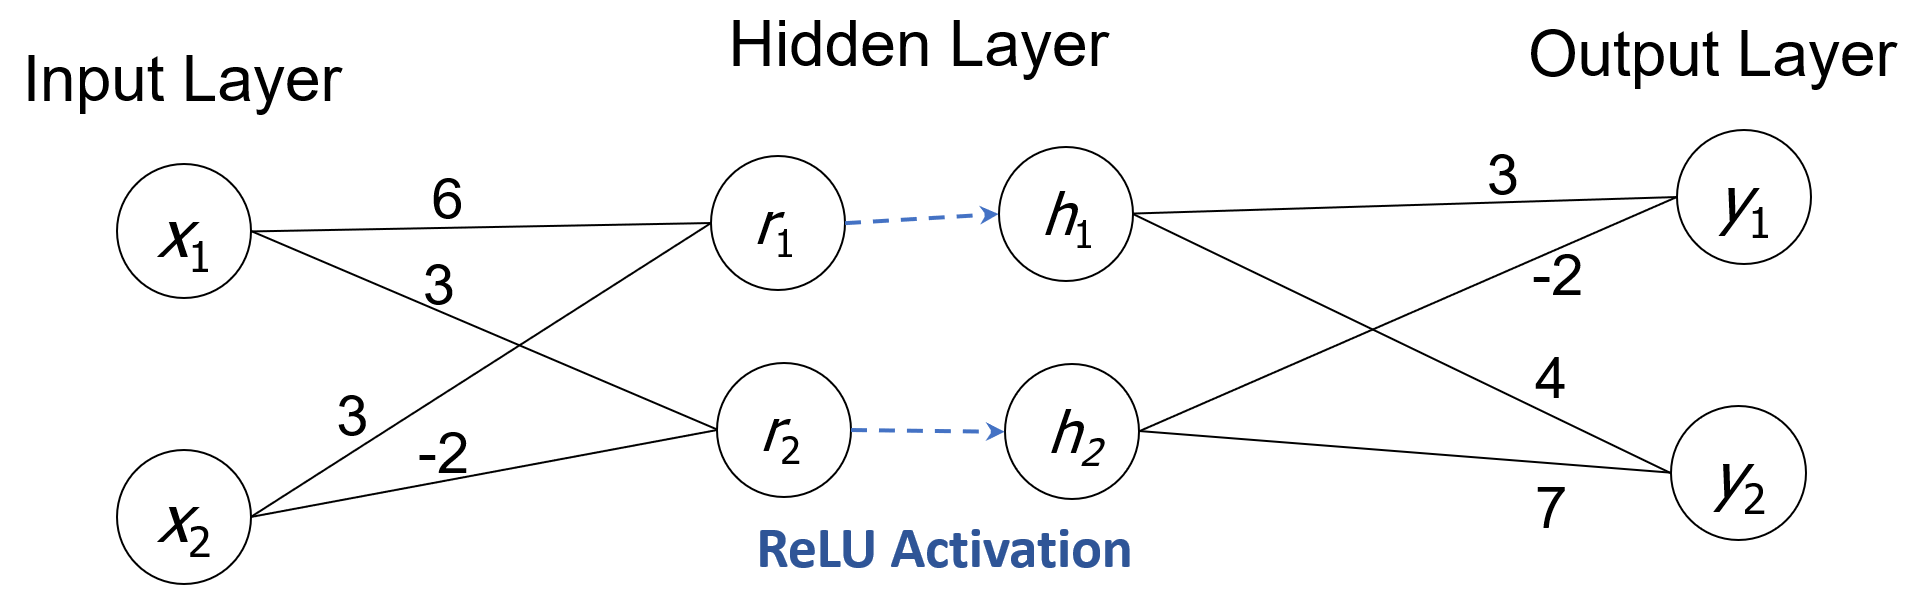
\includegraphics[width=0.8\linewidth]{images/robustnessVerification/q5.PNG}
	\caption{A neural network with one hidden layer with ReLU activation}
	\label{fig-q5}
\end{figure}

\begin{newquestion}{\textbf{5}~~}
\textbf{Lipschitz Continuity}

Given a neural network with one hidden layer with ReLU activation, shown as Figure~\ref{fig-q5}, please prove that the neural network is Lipschitz continuous. Please also calculate the Lipschitz constant of $y_1$ and $y_2$ w.r.t. $x_1$ and $x_2$.

\end{newquestion}



\begin{newquestion}{\textbf{6}~~}\label{q5}
\textbf{Reachability Problem}

Given a neural network with one hidden layer of ReLU activation (shown as Figure~\ref{fig-q5}), assume $x_1\in [3,6.5]$ and $x_2\in [2.5, 5.5]$, what is the output range of $y_1$ and $y_2$?

\begin{itemize}
    \item[1.] Please show how to solve the above reachability problem step by step using MILP/LP.
    
    \item[2.] Please show how to solve the above reachability problem step by step using global optimisation (i.e., DeepGO).
\end{itemize}
\end{newquestion}


\begin{newquestion}{\textbf{7}~~}
\textbf{Verification}

Based on the solution of Question~6,  show how to verify if $y_1\leq y_2$ given $x_1\in [3,6.5]$ and $x_2\in [2.5, 5.5]$?

\end{newquestion}
%%%%%%%%%%%%%%%%%%%%%%%%%%%%%%




\begin{newquestion}{\textbf{8}~~}
Understand the basic idea of adversarial training, and implement an adversarial training algorithm with different step size, number of steps, epoch, to see which hyper-parameter setting can achieve the best balance between performance and running time.  
\end{newquestion}



\begin{newquestion}{\textbf{9}~~}
Does adversarial training compromise the model's  clean accuracy? If so, how to mitigate it?  
\end{newquestion}



\begin{newquestion}{\textbf{10}~~}
Explore different assumptions on the distribution of random weights of DNNs, and understand which assumption is more reasonable in the PAC Bayesian theoretical framework. 
\end{newquestion}



\begin{newquestion}{\textbf{11}~~}
Figure out other technologies to improve generalisation performance of DNNs. 
\end{newquestion}